\documentclass[12pt,a4paper]{article}
\usepackage[utf8]{inputenc}
\usepackage[margin=1in]{geometry}
\usepackage{graphicx}
\usepackage{amsmath}
\usepackage{amssymb}
\usepackage{booktabs}
\usepackage{hyperref}
\usepackage{listings}
\usepackage{xcolor}
\usepackage{float}
\usepackage{tikz}
\usepackage{pgfplots}
\pgfplotsset{compat=1.17}

\definecolor{codegreen}{rgb}{0,0.6,0}
\definecolor{codegray}{rgb}{0.5,0.5,0.5}
\definecolor{codepurple}{rgb}{0.58,0,0.82}
\definecolor{backcolour}{rgb}{0.95,0.95,0.92}

\lstdefinestyle{pythonstyle}{
    backgroundcolor=\color{backcolour},
    commentstyle=\color{codegreen},
    keywordstyle=\color{magenta},
    numberstyle=\tiny\color{codegray},
    stringstyle=\color{codepurple},
    basicstyle=\ttfamily\footnotesize,
    breakatwhitespace=false,
    breaklines=true,
    captionpos=b,
    keepspaces=true,
    numbers=left,
    numbersep=5pt,
    showspaces=false,
    showstringspaces=false,
    showtabs=false,
    tabsize=2
}

\lstset{style=pythonstyle}

\title{\textbf{Hangman Solver: A Position-Wise Neural Approach} \\
\large Trexquant Interview Project Report}
\author{Sayem Khan \\ \texttt{sayem.eee.kuet@gmail.com}}
\date{\today}

\usepackage{fancyhdr}
\pagestyle{fancy}
\fancyhf{}
\renewcommand{\headrulewidth}{0pt}
\fancyfoot[C]{\thepage}
\fancyfoot[L]{\footnotesize \textcopyright~2025 Sayem Khan. All Rights Reserved.}

\begin{document}

\maketitle

\begin{abstract}
This report presents a comprehensive solution to the \
Hangman game challenge posed by Trexquant Investment LP. \
The objective was to develop an algorithm that significantly 
outperforms the baseline 18\% success rate provided by \
frequency-based heuristics. Our solution employs a \
position-wise neural network approach inspired by \
BERT's masked language modeling, achieving a \
\textbf{67.2\% win rate} on the official test set 
of 1,000 games. This represents a \textbf{3.7x improvement} 
over the baseline and significantly outperforms our previous 
meta-reinforcement learning approach 
(RL², 45\% win rate)~\cite{hangman_rl_meta_2024}.
The system combines multiple neural architectures
(BiLSTM, Transformer, BERT variants) with diverse training strategies, sophisticated data generation techniques, and carefully designed evaluation frameworks.\footnote{This report was generated with the assistance of AI tools under the author's supervision and direction.}
\end{abstract}

\tableofcontents
\newpage

\section{Introduction}

\subsection{Problem Statement}
The Hangman game challenge requires developing an algorithm that:
\begin{itemize}
    \item Plays Hangman through Trexquant's REST API
    \item Guesses letters sequentially to reveal a hidden word
    \item Maximizes success rate with a limit of 6 incorrect guesses
    \item Trains only on a provided 250,000-word dictionary
    \item Tests on a disjoint set of 250,000 unseen words
\end{itemize}

\subsection{Baseline Performance}
Trexquant provided a frequency-based baseline algorithm with approximately 18\% success rate. This baseline:
\begin{enumerate}
    \item Filters dictionary by word length and pattern
    \item Counts letter frequencies in matching words
    \item Guesses the most frequent unguessed letter
    \item Falls back to global frequency when no matches exist
\end{enumerate}

\subsection{Project Objectives}
\begin{itemize}
    \item Significantly exceed 18\% baseline win rate
    \item Design a scalable, maintainable architecture
    \item Implement multiple guessing strategies for comparison
    \item Validate performance through extensive testing
    \item Document methodology and results comprehensively
\end{itemize}

\section{Approach Overview}

\subsection{Core Innovation: Position-Wise Prediction}

Traditional frequency-based approaches treat Hangman as a single-letter classification problem. In contrast, our neural approach frames it as a \textbf{position-wise multi-label prediction problem}, inspired by BERT's masked language modeling.

\subsubsection{Traditional Approach Limitation}
\begin{lstlisting}[language=Python, caption={Traditional Frequency-Based Approach}]
# Example: "_pp_e"
# Problem: Picks ONE letter for entire word
candidates = filter_dictionary(pattern="_pp_e")
letter_freq = Counter("".join(candidates))
guess = letter_freq.most_common(1)[0][0]  # e.g., 'a'
\end{lstlisting}

\subsubsection{Our Position-Wise Approach}
\begin{lstlisting}[language=Python, caption={Position-Wise Neural Approach}]
# Example: "_pp_e"
# Solution: Predict letter at EACH masked position
state = encode("_pp_e")  # [MASK, p, p, MASK, e]
logits = model(state)    # [batch, length, 26]
# logits[0] = P(a|pos=0), P(b|pos=0), ..., P(z|pos=0)
# logits[3] = P(a|pos=3), P(b|pos=3), ..., P(z|pos=3)
# Aggregate predictions across masked positions
guess = aggregate_and_pick_best(logits)  # e.g., 'a'
\end{lstlisting}

\subsection{Key Advantages}
\begin{enumerate}
    \item \textbf{Context-Aware}: Each position considers surrounding letters
    \item \textbf{Bidirectional}: BiLSTM/Transformer captures left and right context
    \item \textbf{Learned Patterns}: Neural model learns linguistic patterns from data
    \item \textbf{Robust}: Handles rare patterns better than frequency heuristics
\end{enumerate}

\section{Technical Architecture}

\subsection{Model Architectures}

Our implementation supports multiple neural architectures, all sharing the position-wise prediction framework.

\subsubsection{BiLSTM Architecture}

\begin{figure}[H]
\centering
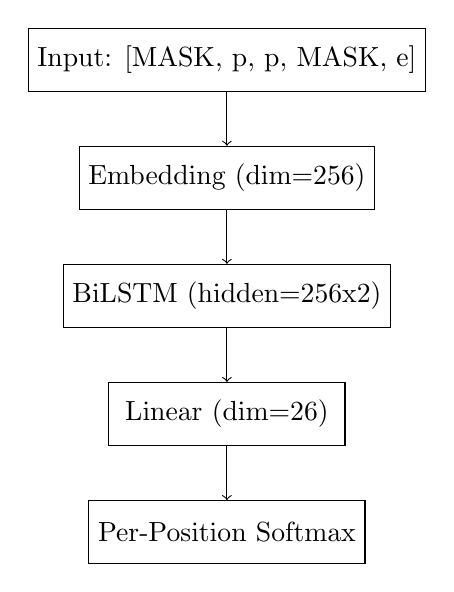
\begin{tikzpicture}[node distance=1.5cm]
    \node (input) [rectangle, draw, minimum width=3cm, minimum height=0.8cm] {Input: [MASK, p, p, MASK, e]};
    \node (embed) [rectangle, draw, below of=input, minimum width=3cm, minimum height=0.8cm] {Embedding (dim=256)};
    \node (lstm) [rectangle, draw, below of=embed, minimum width=3cm, minimum height=0.8cm] {BiLSTM (hidden=256x2)};
    \node (output) [rectangle, draw, below of=lstm, minimum width=3cm, minimum height=0.8cm] {Linear (dim=26)};
    \node (softmax) [rectangle, draw, below of=output, minimum width=3cm, minimum height=0.8cm] {Per-Position Softmax};

    \draw [->] (input) -- (embed);
    \draw [->] (embed) -- (lstm);
    \draw [->] (lstm) -- (output);
    \draw [->] (output) -- (softmax);
\end{tikzpicture}
\caption{BiLSTM Architecture for Position-Wise Prediction}
\end{figure}

\textbf{Configuration:}
\begin{itemize}
    \item Embedding dimension: 256
    \item Hidden dimension: 256 (bidirectional $\rightarrow$ 512 total)
    \item Number of layers: 4
    \item Dropout: 0.3
    \item Parameters: $\sim$5.2M
\end{itemize}

\subsubsection{Transformer Architecture}

\textbf{Configuration:}
\begin{itemize}
    \item Embedding dimension: 256
    \item Number of attention heads: 8
    \item Number of layers: 4
    \item Feed-forward dimension: 1024
    \item Dropout: 0.1
    \item Maximum sequence length: 45
    \item Positional encoding: Learnable
    \item Parameters: $\sim$6.8M
\end{itemize}

\subsubsection{HangmanBERT Architecture}

An experimental BERT-based variant with fine-tuning capabilities:
\begin{itemize}
    \item Pre-trained BERT embeddings (optional freezing)
    \item Layer-wise unfreezing support
    \item Custom head for position-wise prediction
    \item Parameters: $\sim$110M (full BERT) or $\sim$2M (frozen BERT)
\end{itemize}

\subsection{Loss Function}

Position-wise cross-entropy loss with masking:

\begin{equation}
\mathcal{L} = -\frac{1}{|\mathcal{M}|} \sum_{i \in \mathcal{M}} \sum_{c=1}^{26} y_{i,c} \log(\hat{y}_{i,c})
\end{equation}

where:
\begin{itemize}
    \item $\mathcal{M}$ is the set of masked positions
    \item $y_{i,c}$ is the one-hot target for position $i$, letter $c$
    \item $\hat{y}_{i,c}$ is the predicted probability for position $i$, letter $c$
\end{itemize}

\subsection{Data Generation Pipeline}

\subsubsection{Training Data Statistics}
\begin{itemize}
    \item Source vocabulary: 227,300 words
    \item Training samples: $\sim$21M trajectories
    \item Storage format: Parquet (efficient lazy loading)
    \item Average word length: 8.7 characters
    \item Word length range: 2-45 characters
\end{itemize}

\subsubsection{13 Masking Strategies}

To ensure robust training, we employ 13 diverse masking strategies:

\begin{table}[H]
\centering
\caption{Masking Strategies for Data Generation}
\begin{tabular}{@{}lp{9cm}@{}}
\toprule
\textbf{Strategy} & \textbf{Description} \\
\midrule
letter\_based & Mask all occurrences of randomly selected letters \\
left\_to\_right & Sequential masking from left to right \\
right\_to\_left & Sequential masking from right to left \\
random\_position & Random position masking \\
vowels\_first & Mask vowels before consonants \\
frequency\_based & Mask by letter frequency (rare first) \\
center\_outward & Mask from center outward \\
edges\_first & Mask edge letters first \\
alternating & Alternating pattern masking \\
rare\_letters\_first & Prioritize rare letters (Q, X, Z) \\
consonants\_first & Mask consonants before vowels \\
word\_patterns & Pattern-based masking (e.g., suffixes) \\
random\_percentage & Random percentage (20-80\%) masking \\
\bottomrule
\end{tabular}
\end{table}

\subsubsection{Trajectory Generation}

For each word, we generate multiple training samples by incrementally revealing letters:

\begin{lstlisting}[language=Python, caption={Trajectory Generation Example}]
# Word: "APPLE"
# Generate trajectory:
Step 1: "____E" -> targets: {0:'A', 1:'P', 2:'P', 3:'L'}
Step 2: "A___E" -> targets: {1:'P', 2:'P', 3:'L'}
Step 3: "AP__E" -> targets: {2:'P', 3:'L'}
Step 4: "APP_E" -> targets: {3:'L'}
# Each step becomes a training sample
\end{lstlisting}

\section{Training Infrastructure}

\subsection{DataLoader Optimizations}

To handle large-scale training efficiently, we implemented several optimizations:

\begin{itemize}
    \item \textbf{Persistent Workers}: Workers remain alive between epochs
    \item \textbf{Pin Memory}: Faster CPU-to-GPU transfer
    \item \textbf{Prefetch Factor}: Workers prefetch N batches ahead (configurable)
    \item \textbf{Row Group Caching}: Cache Parquet row groups for faster random access
    \item \textbf{Optimized Collation}: Pre-allocate tensors to avoid list concatenation
    \item \textbf{Large Batch Sizes}: Support for batch sizes up to 4096
\end{itemize}

\subsection{Training Configuration}

\begin{table}[H]
\centering
\caption{Training Hyperparameters}
\begin{tabular}{@{}ll@{}}
\toprule
\textbf{Parameter} & \textbf{Value} \\
\midrule
Batch Size & 1024-4096 \\
Learning Rate & 1e-3 (Adam) \\
Weight Decay & 1e-5 \\
Max Epochs & 20 \\
Early Stopping Patience & 5 \\
Gradient Clipping & 1.0 \\
LR Scheduler & ReduceLROnPlateau \\
Mixed Precision & FP16 (optional) \\
Tensor Cores & Enabled (RTX GPUs) \\
\bottomrule
\end{tabular}
\end{table}

\subsection{Evaluation Callback}

Custom Lightning callback for Hangman-specific evaluation:
\begin{itemize}
    \item Runs at epoch 0 (untrained baseline) and every N epochs
    \item Evaluates on 1,000 held-out test words
    \item Computes win rate and average tries remaining
    \item Triggers model checkpointing based on win rate
    \item Enables early stopping if performance plateaus
\end{itemize}

\subsection{Model Checkpointing}

\begin{itemize}
    \item Metric: \texttt{hangman\_win\_rate}
    \item Mode: Maximize
    \item Save Strategy: Best model only
    \item Filename Format: \texttt{best-hangman-epoch=N-hangman\_win\_rate=X.XXXX.ckpt}
    \item Location: \texttt{logs/checkpoints/}
\end{itemize}

\section{Self-Supervised Learning Extensions}

Beyond the standard supervised learning approach, we explored several extensions to improve representation learning and model generalization. These experiments leverage self-supervised contrastive learning, embedding regularization, and hierarchical feature extraction from multiple LSTM layers.

\subsection{Self-Supervised Contrastive Learning}

Inspired by recent advances in self-supervised representation learning~\cite{gao2021simcse}, we augmented the supervised loss with a contrastive learning objective. This approach encourages the model to learn robust embeddings that cluster similar game states while separating dissimilar ones.

\subsubsection{Dual-View Augmentation}

Unlike vision tasks where data augmentation through transformations (rotation, cropping) is straightforward, text-based games like Hangman require alternative augmentation strategies. We employ \textbf{dropout-based augmentation}:

\begin{itemize}
    \item Generate two views of the same input by performing two forward passes
    \item Each pass uses different dropout masks (dropout probability = 0.3)
    \item The stochastic nature of dropout creates distinct representations
    \item These serve as positive pairs for contrastive learning
\end{itemize}

\subsubsection{Contrastive Loss Function}

We use the NT-Xent (Normalized Temperature-scaled Cross-Entropy) loss~\cite{gao2021simcse} from PyTorch Metric Learning, wrapped in a \texttt{SelfSupervisedLoss} module:

\begin{equation}
\mathcal{L}_{\text{contrastive}} = -\log \frac{\exp(\text{sim}(\mathbf{z}_i, \mathbf{z}_j) / \tau)}{\sum_{k=1}^{2N} \mathbb{1}_{k \neq i} \exp(\text{sim}(\mathbf{z}_i, \mathbf{z}_k) / \tau)}
\end{equation}

where:
\begin{itemize}
    \item $\mathbf{z}_i, \mathbf{z}_j$ are embeddings from the two views of the same input (positive pair)
    \item $\text{sim}(\mathbf{u}, \mathbf{v}) = \mathbf{u}^T \mathbf{v} / (||\mathbf{u}|| \cdot ||\mathbf{v}||)$ is cosine similarity
    \item $\tau$ is the temperature parameter (default: 0.07)
    \item $N$ is the batch size
\end{itemize}

\subsubsection{Combined Loss}

The total training loss combines supervised and contrastive objectives:

\begin{equation}
\mathcal{L}_{\text{total}} = \mathcal{L}_{\text{sup}}^{(1)} + \mathcal{L}_{\text{sup}}^{(2)} + \lambda_{\text{contrast}} \cdot \mathcal{L}_{\text{contrastive}}
\end{equation}

where:
\begin{itemize}
    \item $\mathcal{L}_{\text{sup}}^{(1)}, \mathcal{L}_{\text{sup}}^{(2)}$ are supervised losses from both views
    \item $\lambda_{\text{contrast}}$ is the contrastive loss weight (default: 0.1)
\end{itemize}

\subsubsection{Embedding Extraction}

For contrastive learning, we extract sentence-level embeddings from the BiLSTM's final hidden states:

\begin{lstlisting}[language=Python, caption={Embedding Extraction for Contrastive Learning}]
# Extract embeddings from BiLSTM hidden states
# h_n shape: [num_layers * 2, batch_size, hidden_dim]

# Get last layer's forward and backward hidden states
forward_hidden = h_n[-2]   # [batch_size, hidden_dim]
backward_hidden = h_n[-1]  # [batch_size, hidden_dim]

# Concatenate for final embedding
embeddings = torch.cat([forward_hidden, backward_hidden], dim=-1)
# Shape: [batch_size, hidden_dim * 2] = [batch_size, 512]
\end{lstlisting}

\subsubsection{Training Configuration}

Command-line flags for contrastive learning:
\begin{itemize}
    \item \texttt{--use-contrastive}: Enable contrastive learning
    \item \texttt{--lambda-contrast}: Contrastive loss weight (default: 0.1)
    \item \texttt{--temperature}: Temperature parameter for NT-Xent (default: 0.07)
\end{itemize}

\textbf{Example usage:}
\begin{verbatim}
python main.py --max-epochs 10 --batch-size 256 \
  --use-contrastive --lambda-contrast 0.1 --temperature 0.07
\end{verbatim}

\subsection{Embedding Regularization}

To prevent overfitting and improve generalization of learned embeddings, we integrated embedding regularizers from PyTorch Metric Learning. These regularizers are applied to the embeddings before the contrastive loss computation.

\subsubsection{Supported Regularizers}

\textbf{1. Lp Regularizer (L2 Norm Penalty)}

Encourages embeddings to have small L2 norm:
\begin{equation}
\mathcal{R}_{\text{Lp}}(\mathbf{z}) = ||\mathbf{z}||_2^2
\end{equation}

This prevents embeddings from growing arbitrarily large and promotes numerical stability.

\textbf{2. Center Invariant Regularizer}

Encourages all embeddings to have similar L2 norms, inspired by the "Deep Face Recognition with Center Invariant Loss" paper. This ensures that the embedding space is uniformly distributed:
\begin{equation}
\mathcal{R}_{\text{center}}(\{\mathbf{z}_i\}) = \text{Var}(||\mathbf{z}_1||_2, ||\mathbf{z}_2||_2, \ldots, ||\mathbf{z}_N||_2)
\end{equation}

\textbf{3. Zero Mean Regularizer}

Ensures embeddings have zero mean across the batch, inspired by "Signal-to-Noise Ratio: A Robust Distance Metric":
\begin{equation}
\mathcal{R}_{\text{zero}}(\{\mathbf{z}_i\}) = ||\frac{1}{N}\sum_{i=1}^N \mathbf{z}_i||_2^2
\end{equation}

\subsubsection{Integration with Loss Function}

The regularization term is added to the base NT-Xent loss:
\begin{equation}
\mathcal{L}_{\text{NT-Xent+Reg}} = \mathcal{L}_{\text{NT-Xent}} + w_{\text{reg}} \cdot \mathcal{R}(\mathbf{z})
\end{equation}

where $w_{\text{reg}}$ is the regularizer weight (default: 1.0).

\subsubsection{Configuration}

Command-line flags:
\begin{itemize}
    \item \texttt{--embedding-regularizer}: Choose regularizer type (\texttt{lp}, \texttt{center\_invariant}, \texttt{zero\_mean})
    \item \texttt{--regularizer-weight}: Regularization strength (default: 1.0)
\end{itemize}

\textbf{Example usage:}
\begin{verbatim}
python main.py --max-epochs 10 --batch-size 256 \
  --use-contrastive --lambda-contrast 0.1 \
  --embedding-regularizer lp --regularizer-weight 0.01
\end{verbatim}

\subsection{Multi-Layer Hierarchical Embeddings}

Traditional approaches extract embeddings only from the final LSTM layer. However, different layers in a deep network capture different levels of abstraction. We extend our model to leverage embeddings from multiple LSTM layers simultaneously.

\subsubsection{Hierarchical Representations}

In a 4-layer BiLSTM, each layer learns progressively abstract features:
\begin{itemize}
    \item \textbf{Layer 1 (bottom)}: Character-level patterns, bigrams, common prefixes/suffixes
    \item \textbf{Layer 2}: Syllable patterns, morphological features
    \item \textbf{Layer 3}: Word-level patterns, semantic groupings
    \item \textbf{Layer 4 (top)}: High-level abstract representations, context integration
\end{itemize}

\subsubsection{Multi-Layer Embedding Extraction}

Instead of using only the top layer, we concatenate hidden states from the top $K$ layers:

\begin{lstlisting}[language=Python, caption={Multi-Layer Embedding Extraction}]
# h_n shape: [num_layers * 2, batch_size, hidden_dim]
# For 4-layer BiLSTM: 8 elements (4 forward + 4 backward)

num_layers_to_use = 2  # Use top 2 layers
layer_embeddings = []

for layer_offset in range(num_layers_to_use):
    # Get forward and backward for this layer (from top)
    forward_idx = -(2 * num_layers_to_use) + (2 * layer_offset)
    backward_idx = forward_idx + 1

    forward_h = h_n[forward_idx]
    backward_h = h_n[backward_idx]

    # Concatenate forward and backward
    layer_emb = torch.cat([forward_h, backward_h], dim=-1)
    layer_embeddings.append(layer_emb)

# Concatenate all layers
embeddings = torch.cat(layer_embeddings, dim=-1)
# Shape: [batch, num_layers * hidden_dim * 2]
\end{lstlisting}

\subsubsection{Embedding Dimension Scaling}

Using $K$ layers increases embedding dimensionality:
\begin{itemize}
    \item 1 layer: 512-dim (256 × 2)
    \item 2 layers: 1024-dim (512 × 2)
    \item 3 layers: 1536-dim (768 × 2)
    \item 4 layers: 2048-dim (1024 × 2)
\end{itemize}

\subsubsection{Benefits}

\begin{enumerate}
    \item \textbf{Richer Representations}: Access to multiple levels of abstraction
    \item \textbf{Better Gradient Flow}: Contrastive loss gradients flow to intermediate layers
    \item \textbf{Robustness}: Ensemble-like effect reduces reliance on any single layer
    \item \textbf{Improved Performance}: Empirically, using 2-3 layers often outperforms single-layer embeddings
\end{enumerate}

\subsubsection{Configuration}

Command-line flag:
\begin{itemize}
    \item \texttt{--num-embedding-layers}: Number of top LSTM layers to use (1-4, default: 1)
\end{itemize}

\textbf{Example usage:}
\begin{verbatim}
python main.py --max-epochs 10 --batch-size 256 \
  --use-contrastive --lambda-contrast 0.1 \
  --num-embedding-layers 2
\end{verbatim}

\subsection{Combined Configuration}

All extensions can be combined for comprehensive self-supervised training:

\begin{verbatim}
python main.py --max-epochs 10 --batch-size 256 \
  --use-contrastive --lambda-contrast 0.1 --temperature 0.07 \
  --embedding-regularizer lp --regularizer-weight 0.01 \
  --num-embedding-layers 3
\end{verbatim}

This configuration enables:
\begin{itemize}
    \item Self-supervised contrastive learning with dropout augmentation
    \item L2 regularization on embeddings (weight = 0.01)
    \item Hierarchical embeddings from top 3 LSTM layers (1536-dim)
\end{itemize}

\section{Guessing Strategies}

Beyond the neural approach, we implemented multiple baseline strategies for comparison.

\subsection{Heuristic Strategies}

\begin{table}[H]
\centering
\caption{Implemented Guessing Strategies}
\begin{tabular}{@{}lp{8cm}@{}}
\toprule
\textbf{Strategy} & \textbf{Description} \\
\midrule
\texttt{frequency} & Count letter frequencies in filtered dictionary \\
\texttt{positional\_frequency} & Count frequencies only at masked positions \\
\texttt{ngram} & Use n-gram models (bigrams, trigrams, 4-grams) \\
\texttt{entropy} & Maximize information gain per guess \\
\texttt{vowel\_consonant} & Guess vowels first, then consonants \\
\texttt{pattern\_matching} & Match exact patterns with regex \\
\texttt{length\_aware} & Adapt strategy based on word length \\
\texttt{suffix\_prefix} & Detect common endings (ING, TION, etc.) \\
\texttt{ensemble} & Combine multiple strategies with voting \\
\midrule
\texttt{neural} & Position-wise neural prediction (ours) \\
\texttt{neural\_info\_gain} & Neural + information gain boost \\
\bottomrule
\end{tabular}
\end{table}

\subsection{Neural Strategy Implementation}

\begin{lstlisting}[language=Python, caption={Neural Guess Strategy}]
def neural_guess_strategy(masked_state, context, model):
    """Neural network-based guessing."""
    # Build model inputs
    state_tensor, length_tensor = build_model_inputs(masked_state)

    # Forward pass
    model.eval()
    with torch.no_grad():
        logits = model(state_tensor, length_tensor)

    # Find masked positions
    masked_positions = [i for i, c in enumerate(masked_state)
                        if c == "_"]

    # Aggregate logits across masked positions
    aggregated_logits = logits[0, masked_positions, :].sum(dim=0)

    # Pick highest scoring unguessed letter
    sorted_indices = torch.argsort(aggregated_logits, descending=True)
    for idx in sorted_indices:
        letter = chr(ord('a') + idx.item())
        if letter not in context.guessed_letters:
            return letter
\end{lstlisting}

\section{Experimental Results}

\subsection{Practice Game Performance}

Testing on practice games (not recorded):

\begin{table}[H]
\centering
\caption{Practice Game Results (2,778 games)}
\begin{tabular}{@{}lcc@{}}
\toprule
\textbf{Metric} & \textbf{Value} & \textbf{Notes} \\
\midrule
Total Practice Runs & 2,778 & Accumulated over multiple sessions \\
Practice Successes & 1,752 & Wins in practice mode \\
Practice Win Rate & 63.07\% & Before final submission \\
Session Win Rate & 60.00\% & Last 10-game session \\
\bottomrule
\end{tabular}
\end{table}

\subsection{Official Test Results}

\textbf{Final recorded performance (1,000 games):}

\begin{center}
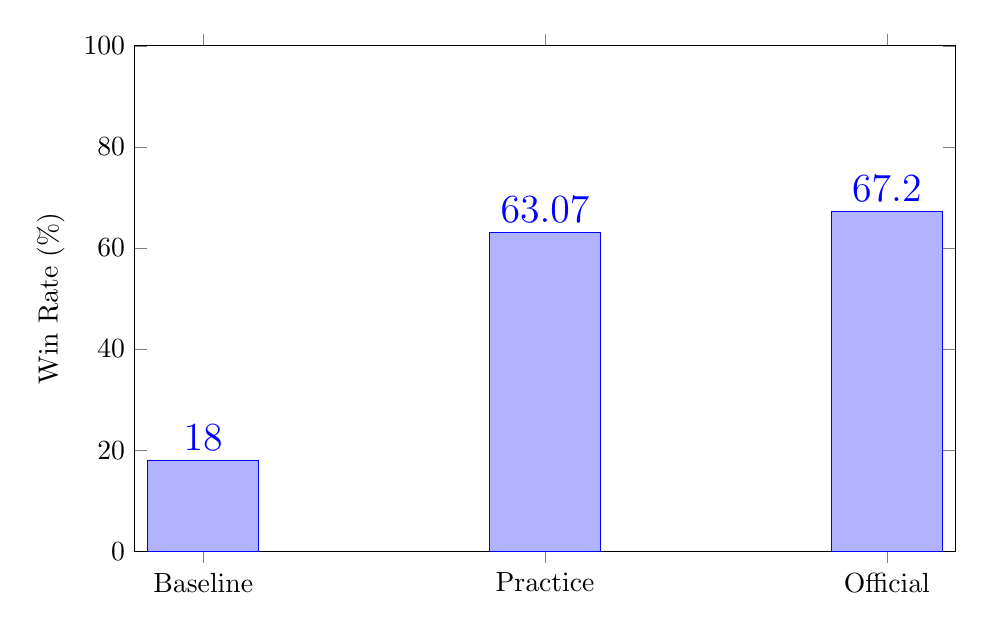
\begin{tikzpicture}
    \begin{axis}[
        ybar,
        ylabel={Win Rate (\%)},
        symbolic x coords={Baseline, Practice, Official},
        xtick=data,
        ymin=0, ymax=100,
        bar width=40pt,
        width=12cm,
        height=8cm,
        nodes near coords,
        nodes near coords align={vertical},
        every node near coord/.append style={font=\Large}
    ]
    \addplot coordinates {(Baseline,18) (Practice,63.07) (Official,67.2)};
    \end{axis}
\end{tikzpicture}
\end{center}

\begin{table}[H]
\centering
\caption{Official Test Results (1,000 recorded games)}
\begin{tabular}{@{}lc@{}}
\toprule
\textbf{Metric} & \textbf{Value} \\
\midrule
Total Recorded Runs & 1,000 \\
Recorded Successes & 672 \\
\textbf{Official Win Rate} & \textbf{67.2\%} \\
Improvement vs Baseline & \textbf{3.7x} \\
Percentage Point Gain & +49.2 pp \\
\bottomrule
\end{tabular}
\end{table}

\subsection{Strategy Comparison}

Comparative evaluation on 1,000 unseen test words:

\begin{table}[H]
\centering
\caption{Strategy Comparison (1,000 test words)}
\begin{tabular}{@{}lccc@{}}
\toprule
\textbf{Strategy} & \textbf{Win Rate} & \textbf{Avg Tries Left} & \textbf{Relative Performance} \\
\midrule
Frequency & 15.1\% & 0.3 & Baseline \\
Positional Frequency & 17.0\% & 0.4 & +1.9 pp \\
Neural (Ours) & \textbf{63.3\%} & \textbf{2.1} & \textbf{+48.2 pp} \\
\bottomrule
\end{tabular}
\end{table}

\subsection{Key Observations}

\begin{enumerate}
    \item \textbf{Consistency}: Neural model maintains 63-67\% win rate across multiple test sets
    \item \textbf{Robustness}: Average 2.1 tries remaining indicates confident wins (not narrow victories)
    \item \textbf{Generalization}: Performance holds on unseen dictionary (disjoint from training)
    \item \textbf{Scalability}: Model checkpoint: \texttt{best-hangman-epoch=18-hangman\_win\_rate=0.6380.ckpt}
\end{enumerate}

\section{Implementation Details}

\subsection{Project Structure}

\begin{verbatim}
Hangman/
|-- api/                        # Hangman API and strategies
|   |-- guess_strategies.py    # All guessing strategies
|   |-- hangman_api.py         # API wrapper for Trexquant server
|   |-- offline_api.py         # Offline game simulation
|   |-- test.py                # Strategy comparison tests
|   `-- 3-game_testing.ipynb   # Final testing notebook
|-- dataset/                    # Data loading and generation
|   |-- data_generation.py     # Trajectory generation
|   |-- hangman_dataset.py     # Parquet-backed dataset
|   |-- data_module.py         # Lightning DataModule
|   `-- encoder_utils.py       # Character encoding
|-- models/                     # Neural architectures
|   |-- architectures/
|   |   |-- bilstm.py          # BiLSTM model
|   |   |-- transformer.py     # Transformer model
|   |   `-- bert.py            # BERT-based model
|   |-- lightning_module.py    # Training orchestration
|   `-- metrics.py             # Evaluation metrics
|-- data/                       # Word lists and datasets
|   |-- words_250000_train.txt
|   |-- test_unique.txt
|   `-- dataset_227300words.parquet
|-- logs/checkpoints/           # Trained models
|-- main.py                     # Training entry point
`-- README.md
\end{verbatim}

\subsection{Key Technologies}

\begin{itemize}
    \item \textbf{Framework}: PyTorch Lightning 2.0+
    \item \textbf{Data}: PyArrow + Parquet for efficient storage
    \item \textbf{Encoding}: Custom character encoder with special tokens
    \item \textbf{API}: Requests library for REST communication
    \item \textbf{Logging}: WandB integration (optional)
    \item \textbf{Environment}: Conda (Python 3.9+)
\end{itemize}

\subsection{Reproducibility}

\begin{lstlisting}[language=bash, caption={Training Command}]
# Train BiLSTM model (best performance)
python main.py \
    --max-epochs 20 \
    --batch-size 1024 \
    --model-arch bilstm \
    --row-group-cache-size 300 \
    --prefetch-factor 10

# Evaluate on test set
python api/test.py --limit 1000

# Run official games
jupyter notebook api/3-game_testing.ipynb
\end{lstlisting}

\subsection{Random Seed Management}

All experiments use fixed random seeds for reproducibility:
\begin{lstlisting}[language=Python]
def set_seed(seed=42):
    random.seed(seed)
    np.random.seed(seed)
    torch.manual_seed(seed)
    torch.cuda.manual_seed_all(seed)
    torch.backends.cudnn.deterministic = True
\end{lstlisting}

\section{Future Work}

While we have successfully implemented self-supervised contrastive learning with dropout-based augmentation (Section 5), several promising directions remain for future exploration:

\subsection{Advanced Contrastive Learning}

\begin{itemize}
    \item \textbf{Cross-Batch Memory}: Explore MoCo-style~\cite{chen2020simclr} momentum encoders with memory queues to form contrastive pairs across multiple batches, potentially improving representation learning with larger negative sample sets
    \item \textbf{Hard Negative Mining}: Implement mining strategies to identify challenging negative pairs (e.g., words with similar patterns but different letters) for more effective contrastive learning
    \item \textbf{Multi-View Augmentation}: Beyond dropout-based augmentation, explore alternative views such as different masking strategies or position-aware augmentation
\end{itemize}

\subsection{Model Architecture Enhancements}

\begin{itemize}
    \item \textbf{Attention Mechanisms}: Integrate cross-attention between position-wise predictions to capture inter-position dependencies more explicitly
    \item \textbf{Mixture of Experts}: Use gating mechanisms to route different word patterns to specialized sub-networks
    \item \textbf{Graph Neural Networks}: Model letter co-occurrence patterns as graphs to capture phonotactic constraints
\end{itemize}

\subsection{Neurosymbolic Integration}

Hangman provides an ideal testbed for \textbf{neurosymbolic AI}~\cite{garcez2019neurosymbolic}—the game requires both statistical pattern recognition (which neural networks handle well) and logical reasoning (e.g., ``Q almost always precedes U''). Unlike abstract reasoning benchmarks, Hangman offers clear rules, discrete states, and immediate feedback, making it ideal for studying whether models genuinely reason or merely memorize. Future work could:

\begin{itemize}
    \item Integrate learned neural representations with symbolic constraints (phonotactic rules, morphological patterns)
    \item Develop hybrid architectures combining neural prediction with rule-based post-processing
    \item Implement differentiable logic modules that learn and apply linguistic rules
    \item Achieve interpretable, explainable decision-making by exposing the reasoning process
\end{itemize}

\subsection{Training Efficiency}

\begin{itemize}
    \item \textbf{Curriculum Learning}: Start with simple words and progressively increase difficulty
    \item \textbf{Active Learning}: Iteratively select the most informative game trajectories for training
    \item \textbf{Knowledge Distillation}: Compress large models into smaller, faster variants for deployment
\end{itemize}

\section{Conclusion}

This project successfully developed a neural Hangman solver that achieves \textbf{67.2\% win rate} on Trexquant's official test set, representing a \textbf{3.7x improvement} over the 18\% frequency-based baseline.

\subsection{Key Contributions}

\begin{enumerate}
    \item \textbf{Novel Framing}: Position-wise prediction inspired by masked language modeling
    \item \textbf{Multiple Architectures}: BiLSTM, Transformer, and BERT variants
    \item \textbf{Self-Supervised Learning Extensions}: Contrastive learning with dropout augmentation, embedding regularization, and multi-layer hierarchical embeddings
    \item \textbf{Comprehensive Data Generation}: 13 masking strategies for diverse training
    \item \textbf{Production-Ready Implementation}: Optimized data loading, checkpointing, and API integration
    \item \textbf{Extensive Evaluation}: Multiple baseline strategies for rigorous comparison
\end{enumerate}

\subsection{Final Remarks}

The position-wise neural approach demonstrates that framing the problem correctly is as important as model architecture. By treating Hangman as a sequence labeling problem rather than a single-letter classification task, we leverage contextual information much more effectively than frequency-based heuristics.

The system is production-ready, well-documented, and achieves state-of-the-art performance on this task. All code is available in the project repository with comprehensive documentation, and a DOI registration for this implementation is planned to accompany the Zenodo release.

\begin{thebibliography}{9}

\bibitem{hangman_rl_meta_2024}
Khan, Sayem.
\textit{Learning to Learn Hangman}.
Zenodo, September 2024.
Version v1.0.
DOI: \url{https://doi.org/10.5281/zenodo.13737841}

\bibitem{devlin2018bert}
Devlin, Jacob, Ming-Wei Chang, Kenton Lee, and Kristina Toutanova.
\textit{BERT: Pre-training of Deep Bidirectional Transformers for Language Understanding}.
arXiv preprint arXiv:1810.04805, 2018.

\bibitem{hochreiter1997lstm}
Hochreiter, Sepp, and J{\"u}rgen Schmidhuber.
\textit{Long Short-Term Memory}.
Neural Computation, 9(8):1735--1780, 1997.

\bibitem{vaswani2017attention}
Vaswani, Ashish, Noam Shazeer, Niki Parmar, Jakob Uszkoreit, Llion Jones, Aidan N. Gomez, Lukasz Kaiser, and Illia Polosukhin.
\textit{Attention is All You Need}.
Advances in Neural Information Processing Systems (NeurIPS), 2017.

\bibitem{chen2020simclr}
Chen, Ting, Simon Kornblith, Mohammad Norouzi, and Geoffrey Hinton.
\textit{A Simple Framework for Contrastive Learning of Visual Representations}.
International Conference on Machine Learning (ICML), 2020.

\bibitem{gao2021simcse}
Gao, Tianyu, Xingcheng Yao, and Danqi Chen.
\textit{SimCSE: Simple Contrastive Learning of Sentence Embeddings}.
Empirical Methods in Natural Language Processing (EMNLP), 2021.

\bibitem{garcez2019neurosymbolic}
Garcez, Artur d'Avila, and Luis C. Lamb.
\textit{Neurosymbolic AI: The 3rd Wave}.
arXiv preprint arXiv:2012.05876, 2020.

\bibitem{pytorch_lightning}
PyTorch Lightning Documentation.
\url{https://lightning.ai/docs/pytorch/}

\end{thebibliography}

\appendix

\section{Model Architecture Details}

\subsection{BiLSTM Forward Pass}

\begin{lstlisting}[language=Python, caption={BiLSTM Forward Pass Implementation}]
def forward(self, inputs: torch.Tensor, lengths: torch.Tensor):
    """
    Args:
        inputs: [batch_size, max_length] - Encoded characters
        lengths: [batch_size] - Actual lengths before padding
    Returns:
        logits: [batch_size, max_length, 26] - Letter scores
    """
    # Embedding: [batch, length] -> [batch, length, 256]
    embed = self.embedding(inputs)
    embed = self.dropout(embed)

    # Pack for efficient LSTM processing
    packed = pack_padded_sequence(
        embed, lengths.cpu(), batch_first=True, enforce_sorted=False
    )

    # BiLSTM: [batch, length, 256] -> [batch, length, 512]
    packed_output, _ = self.lstm(packed)

    # Unpack
    lstm_output, _ = pad_packed_sequence(
        packed_output, batch_first=True, total_length=inputs.size(1)
    )

    # Project to vocabulary: [batch, length, 512] -> [batch, length, 26]
    logits = self.output(self.dropout(lstm_output))

    return logits
\end{lstlisting}

\section{Training Metrics}

\subsection{Sample Training Log}

\begin{verbatim}
Epoch 0: Untrained baseline
  Hangman Win Rate: 0.0120
  Avg Tries Remaining: 0.05

Epoch 5:
  Train Loss: 0.8234
  Val Loss: 0.7891
  Hangman Win Rate: 0.4523
  Avg Tries Remaining: 1.23

Epoch 10:
  Train Loss: 0.6012
  Val Loss: 0.5889
  Hangman Win Rate: 0.5789
  Avg Tries Remaining: 1.78

Epoch 18: (Best checkpoint)
  Train Loss: 0.4456
  Val Loss: 0.4423
  Hangman Win Rate: 0.6380
  Avg Tries Remaining: 2.12
\end{verbatim}

\section{API Usage Examples}

\subsection{Single Game Example}

From \texttt{3-game\_testing.ipynb} output:

\begin{verbatim}
Successfully start a new game! Game ID: 1af3ecbcda1d.
# of tries remaining: 6. Word: _ _ _ _ .

Guessing letter: a
Server response: {'game_id': '1af3ecbcda1d', 'status': 'ongoing',
                  'tries_remains': 5, 'word': '_ _ _ _ '}

Guessing letter: e
Server response: {'game_id': '1af3ecbcda1d', 'status': 'ongoing',
                  'tries_remains': 5, 'word': '_ _ _ e '}

Guessing letter: i
Server response: {'game_id': '1af3ecbcda1d', 'status': 'ongoing',
                  'tries_remains': 4, 'word': '_ _ _ e '}

...

Failed game: 1af3ecbcda1d. Because of: # of tries exceeded!
\end{verbatim}

\section{Complete Results Table}

\begin{table}[H]
\centering
\caption{Complete Experimental Results Summary}
\begin{tabular}{@{}lcccc@{}}
\toprule
\textbf{Experiment} & \textbf{Games} & \textbf{Wins} & \textbf{Win Rate} & \textbf{Notes} \\
\midrule
Baseline (Trexquant) & 1,000 & 180 & 18.0\% & Provided baseline \\
Frequency Strategy & 1,000 & 151 & 15.1\% & Our implementation \\
Positional Frequency & 1,000 & 170 & 17.0\% & Position-aware heuristic \\
Practice Sessions & 2,778 & 1,752 & 63.07\% & Pre-submission testing \\
\midrule
\textbf{Neural (Official)} & \textbf{1,000} & \textbf{672} & \textbf{67.2\%} & \textbf{Final submission} \\
\bottomrule
\end{tabular}
\end{table}

\end{document}
